%TCIDATA{LaTeXparent=0,0,relatorio.tex}
\ifx\compilewholereport\undefined
	\documentclass[11pt,a4paper,oneside]{book}
	
	% Escolher um dos seguintes formatos:
	\usepackage{ft2unb} % segue padrão de fontes do Latex
	
	% Pacotes
	\usepackage{graphicx}
	\usepackage{amsfonts}
	\usepackage{amsmath}
	\usepackage{amssymb}
	\usepackage[thmmarks,amsmath]{ntheorem}
	\usepackage{boxedminipage}
	\usepackage{theorem}
	\usepackage{fancybox}
	\usepackage{fancyhdr}
	\usepackage{url}
	\usepackage{afterpage}
	\usepackage{color}
	\usepackage{colortbl}
	\usepackage{rotating}
	\usepackage{makeidx}
	\usepackage{indentfirst}
	\usepackage{bibentry}
	\usepackage{subcaption}
	\usepackage{todonotes}
	\presetkeys{todonotes}{inline}{}
	
	\begin{document}
	\frontmatter
	\tableofcontents
	\mainmatter
	
	%%%%%%%%%%%%%%%%%%%%%%%%%%%%
	%%%%%%%% Apagar coisas acima
	%%%%%%%%%%%%%%%%%%%%%%%%%%%%
	\newcommand\qt[1]{\lq\lq{}#1\rq\rq{}}
	\newcommand\qti[1]{\lq\lq{}\textit{#1}\rq\rq{}}
\fi
                      
\chapter{Revis\~{a}o Bibliogr\'{a}fica}\label{CapRevisaoBibliografica}

% Resumo opcional. Comentar se não usar.
\resumodocapitulo{Este capítulo visa apresentar uma breve descrição sobre reconfiguração dinâmica, autorreconfiguração e as ferramentas e conceitos necessários para o seu entendimento.}

\section{Compilação de \textit{Hardware}}
A compilação de \textit{hardware} é um processo primordial no desenvolvimento de sistemas reconfiguráveis, equivalente à compilação para projetos de \textit{software} \cite{Hauck2007}.
A figura \ref{fig:sintese} apresenta duas imagens que apresentam este processo de compilação.

\begin{figure}[h]
	\centering
       	\begin{subfigure}[b]{0.4\textwidth}
       		\centering
		\includegraphics[width=\textwidth]{fig/c1_introducao/sintese_simples.pdf}
		\caption{Imagem ilustrativa do fluxo de compilação de um projeto de \textit{hardware}, extraida de \cite{Hauck2007}.}
		\label{fig:sintese_simples}
	\end{subfigure}\quad
	\begin{subfigure}[b]{0.55\textwidth}
		\centering
		\includegraphics[width=\textwidth]{fig/c1_introducao/sintese.pdf}
		\caption{Imagem ilustrativa do fluxo de compilação de um projeto de \textit{hardware} segundo visto pelo usuário, extraida de \cite{Hauck2007}.}
		\label{fig:sintese_user}
	\end{subfigure}
	\caption{Imagens do fluxo da compilação de \textit{hardware}.}
	\label{fig:sintese}
\end{figure}

\paragraph{Descrição}
Assim como no \textit{software},  se inicia com a descrição do funcionamento do sistema.
Esta descrição em geral é feita utilizando-se especificações de um problema/aplicação.
Ela pode ser realizada em Verilog, VDHL e diagramas de blocos, na maioria dos casos.
Utiliza-se ainda a simulação funcional, como mostrado na figura \ref{fig:sintese_user}, para validar a descrição realizada.

\paragraph{Síntese Lógica}
A partir do código fonte construido, realiza-se a síntese lógica, processo que consiste em transformar a descrição comportamental ou estrutural em elementos lógicos \cite{Thomas1996, Ashenden2008}.
Assim como na compilação de \textit{software}, existe uma fase de pré-processamento que expande macros, inclui arquivos e realiza a verificação léxica e sintática da descrição.
Diversos algoritmos de otimização também são aplicados de forma a reduzir as equações lógicas, otimizando seu espaço no dispositivo e performance.

\paragraph{Colocação (\textit{Placement}) e Roteamento (\textit{Routing})}
A colocação, que aqui também abrange a etapa de \textit{floorplanning}, consiste em identificar onde a lógica deverá ser posicionada para satisfazer os requisitos de tempo, potência e performance, segundo as limitações do dispositivo-alvo.
Ela recebe informações da lógica do projeto e dos recursos lógicos do dispositivo e aplica algoritmos de otimização para alcançar todos os objetivos e pré-requisitos impostos.

A etapa de roteamento, em conjunto com a colocação, tenta conectar os elementos necessários de acordo com as limitações do FPGA.
Para projetos grandes, com muitos elementos lógicos, pode ser muito dificil, tornando o processo lento, ou até impossível de se realizar esta etapa.
Note que o roteamente interfere diretamente com questões relacionadas a tempo e performance.

\paragraph{Análise e Simulação de \textit{Timing}}
Durante a colocação e o roteamento, várias informações de tempo do projeto são calculados e associados ao projeto.
Após estas etapas, uma análise estática de temporização e simulações extremamente precisas podem ser realizadas, removendo todas as dúvidas quanto ao projeto realizado e as descrições impostas.

\paragraph{Geração do Arquivo Binário (\textit{Bitstream Generation})}
A etapa de geração do arquivo binário corresponde a transformação das informações geradas na síntese, na colocação e no roteamento para bits de programação da FPGA.
Estes bits popularão, durante a fase de programação, as LUTs e RAMs da placa, definindo seu funcionamento.

\section{\textit{Benchmark}}
A avaliação de desempenho de sistemas reconfiguráveis não pode mais ser dada com base em quantidade de operações em ponto flutuante (FLOPS) como é feita em computadores e similares \cite{patterson2005coa, cullinan2012computing}.
A melhor forma de se comparar dispositivos é através de do uso de uma mesma aplicação sintetizada com as ferramentas específicas de cada empresa.
Neste caso, pórem, a comparação também leva em consideração o desempenho das ferramentas, especialmente em sua capacidade de otimizar as funções implementadas.
Outra forma comum de se comparar desempenho é específico através de uma análise de aplicações específicas.
Um exemplo para uma aplicação de filtragem de imagens é a quantidade de quadros ela consegue processar em um determinado periodo de tempo.

\section{Dispositivos}
As formas mais comuns de dispositivos reconfigur\'aveis s\~ao o \textit{Programmable Array Logic} (PAL), o \textit{Complex Programmable Logic Device} (CPLD), o \textit{Field-Programmable Gate Array} e o \textit{Reconfigurable Datapath Array} (rDPA).
Cada um possui suas vantagens e desvantagens segundo a forma de implementa\c{c}\~ao, comentadas a seguir.

\begin{figure}[h]
\centering
\includegraphics[width=0.7\textwidth]{fig/c1_introducao/model_pal.pdf}
\caption{Circuito interno de um dispositivo do tipo PAL, extraido de \cite{Ashenden2008}.}
\label{fig:pal}
\end{figure}

\subsection{\textit{Programmable Array Logic}}
Os \textit{Programmable Array Logics} (PALs) foram os primeiros dispositivos program\'aveis, desenvolvidos por volta de 1970.
Os PALs podem ser configurados para desempenhar diversas fun\c{c}\~oes l\'ogicas com possibilidade de cascateamento.
Alguns tipos especiais de PALs tamb\'em cont\'em registradores, permitindo a programa\c{c}\~ao de circuitos sequenciais simples.
Outra caracter\'i­stica dos PALs que permitiam a constru\c{c}\~ao de circuitos l\'ogicas um pouco mais complexas era a realimenta\c{c}\~ao, como pode ser visto na figura \ref{fig:pal}.
Eles podem ser programados usando uma linguagem de descri\c{c}\~ao de \textit{hardware} com informa\c{c}\~oes na forma de express\~oes booleanas.
Eles por\'em se tornaram obsoletos com a chegada dos \textit{Generic Array Logics} (GALs) e \textit{Complex Programmable Logic Devices} (CPLDs).
Eles eram produzidos principalmente pela Data I/O Corporation.

Os PALs surgiram para substituir a l\'ogica TTL, usada em granda escala na prototipagem e em dispositivos pequenos.
Em geral, mesmo que para projetos com apenas alguns elementos de l\'ogica TTL, o uso de PALs possu\'i­a um custo e confiabilidade maiores que na combina\c{c}\~ao de v\'arios \textit{chips} diferentes.
Sua programa\c{c}\~ao \'e feita atrav\'es de conex\~oes compostas por pequenos fus\'i­veis, que s\~ao queimados quando a conex\~ao n\~ao \'e necess\'aria.

\begin{figure}[h]
\centering
\includegraphics[width=0.5\textwidth]{fig/c1_introducao/model_cpld.pdf}
\caption{Representa\c{c}\~ao de dispositivos do tipo CPLD, extraido de \cite{Ashenden2008}.}
\label{fig:cpld}
\end{figure}

\subsection{\textit{Complex Programmable Logic Device}}
Desenvolvida depois dos PALs, os CPLDs s\~ao dispositivos similares aos PALs, mas com suporte a um n\'umero maior de blocos l\'ogicos.
Eles podem ser definidos como um conjundo de PALs conectados por uma rede program\'avel de conex\~oes, como tenta esquematizar a figura \ref{fig:cpld}.
Sua arquitetura \'e baseada no mar de portas, como mostra a figura \ref{fig:cpld}.
Detalhes de implementa\c{c}\~ao variam de fabricante.

Al\'em de conter mais recursos que os PALs, os CPLDs s\~ao diferentes na forma de programa\c{c}\~ao.
Ao inv\'es de usar EEPROM, eles usam mem\'orias RAM n\~ao-vol\'ateis para armazenar a programa\c{c}\~ao quando o sistema \'e desligado e c\'elulas de mem\'oria SRAM para armazenar as informa\c{c}\~oes de conex\~oes e comportamento das c\'elulas l\'ogicas.
Quando o dispositivo \'e energizado, a programa\c{c}\~ao da mem\'oria RAM \'e passada para as c\'elulas SRAM, que permitem que o sistema funcione.
A mem\'oria n\~ao-vol\'atil tamb\'em possui pinos independentes acess\'i­veis externamente, o que permitem que ele seja programado mesmo depois de soldado ao produto final permitindo sua atualiza\c{c}\~ao.

A maior vantagem dos CPLDs com rela\c{c}\~ao a outros dispositivos \'e a sua n\~ao-volatilidade, tornando-o muito \'util como \textit{bootloaders} ou em aplica\c{c}\~oes que precisem rodar assim que o sistema \'e energizado.
O mais famoso destes dispositivos, conhecido por Max, \'e desenvolvido pela Altera.

\begin{figure}[h]
\centering
\includegraphics[width=0.65\textwidth]{fig/c1_introducao/model_fpga.pdf}
\caption{Representa\c{c}\~ao de dispositivos do tipo FPGA, extraido de \cite{Ashenden2008}.}
\label{fig:fpga}
\end{figure}

\subsection{\textit{Field-Programmable Gate Array}}
Formado de c\'elulas program\'aveis consideravelmente menores que as dos CPLDs, que permitem uma maior integra\c{c}\~ao, existe o \textit{Field-Programmable Gate Array}.
Como se pode notar, este dispositivo possui dentre as suas caracter\'i­sticas principais a capacidade de ser programado e reprogramado em campo (\textit{field}), isto \'e, sem a necessidade de processos especiais.
Apesar disso, devido a complexidade dos circuitos internos destes dispositivos, simplificados na figura \ref{fig:fpga}, eles n\~ao foram feitos para serem programados manualmente, o que ainda era poss\'i­vel com os CPLDs, fazendo-se necess\'ario o uso de ferramentas de projeto auxiliado por computador (CAD) para, dado um c\'odigo em linguagem de descri\c{c}\~ao de \textit{hardware}, sintetizar, mapear, alocar e rotear o projeto automaticamente.

Desde a sua inven\c{c}\~ao, as FPGAs vem crescendo em capacidade e performance, tendo se tornado o principal componente de computa\c{c}\~ao reconfigur\'avel.
A maioria das suas implementa\c{c}\~oes se assemelha, em alto n\'i­vel, ao circuito apresentado na figura \ref{fig:fpga}.
Eles incluem blocos l\'ogicos que podem implementar tanto l\'ogicas combinacionais simples quanto fun\c{c}\~oes l\'ogicas sequenciais, blocos de entrada e sa\'i­da registrados ou n\~ao com possibilidade de funcionamento em diversos n\'i­veis l\'ogicos e condi\c{c}\~oes de temporiza\c{c}\~ao, c\'elulas de mem\'oria RAM embutidas e uma rede de conex\~oes program\'avel.
A raz\~ao para permitir que todas estas caracter\'i­sticas sejam programadas \'e permitir que os FPGAs sejam usados nos mais diversos tipos de sistemas, que usam diferentes padr\~oes de sinais entre \textit{chips}.
Detalhes de implementa\c{c}\~ao por\'em variam entre fabricantes e fam\'i­lias de dispositivos.
Apesar disso, em sua maioria, utilizam de mem\'orias RAM ass\'i­ncronas de 1 bit conhecidas como \textit{lookup tables} (LUTs), al\'em de \textit{flip-flops} e multiplexadores.
Algumas FPGAs tamb\'em incluem c\'elulas especializadas de processamento como multiplicadores e processadores gen\'ericos.

Existem dois tipos de FPGAs, um baseado em mem\'oria RAM e outro baseado em \textit{antifuses}.
Como foi falado na se\c{c}\~ao \ref{ss:computacao_reconfiguravel}, a mem\'oria RAM \'e vol\'atil, for\c{c}ando o sistema a ser programado toda vez que energizado.
Apesar disso, possui a vantagem de poder ter sua programa\c{c}\~ao modificada em campo.
O FPGA baseado em \textit{antifuses} s\'o pode ser programado uma vez, na f\'abrica.

\begin{table}[h]
\centering
\begin{tabular}{|c|c|c|c|}
\hline
 & PAL & CPLD & FPGA \\ \hline
Custo & \$2-\$15 & \$5-\$50 & \$10-\$300 \\ \hline
Blocos l\'ogicos & 8-10 & 32 - 128 & 100+ \\ \hline
Pinos de I/O & 20-24 & 44-160 & 84-256\\ \hline
Configura\c{c}\~ao & EEPROM & EEPROM & RAM ou OTP\\ \hline
Projeto & Equa\c{c}\~oes Booleanas & HDL ou esquem\'atico & HDL ou esquem\'atico\\ \hline
\end{tabular}
\caption{Tabela comparativa dos dipositivos reconfigur\'aveis dos tipos PAL, CPLD e FPGA.}
\label{tab:comparacao}
\end{table}

A tabela \ref{tab:comparacao} apresenta uma compara\c{c}\~ao ligeiramente grosseira entre os PALs, CPLDs e FPGAs.

\begin{figure}[h]
\centering
\includegraphics[width=0.5\textwidth]{fig/c1_introducao/model_rdpa.pdf}
\caption{Modelo de rDPA do tipo KressArray-I, extraido de \cite{Hartenstein1995}.}
\label{fig:kressarray}
\end{figure}

\subsection{\textit{Reconfigurable Datapath Array}}
O \textit{Reconfigurable Datapath Array} \'e um tipo de sistema reconfigur\'avel com granularidade grossa, normalmente 32 bits \cite{Hartenstein2001}.
Apesar de relativamente mais novo que os dispositivos abaixo, ele \'e menos utilizado.
Seus blocos l\'ogicos, chamados de \textit{datapath processing units} (DPUs), s\~ao um pouco mais complexos que os dispositivos de granularidade fina de forma a conseguir tratar os dados maiores.
Eles possuem m\'ultiplas conex\~oes uni e birecionais entre seus vizinhos diretos, al\'em de trilhas verticais/horizontais completas ou segmentadas e um trilha principal mais externa que conecta todos os blocos, conforme mostra a figura \ref{fig:kressarray}.
As vantagens deste tipo de sistema reconfigur\'avel s\~ao um maior poder de processamento para uma mesma complexidade de roteamento em rela\c{c}\~ao aos sistemas de granularidade mais fina al\'em de um tempo de configura\c{c}\~ao reduzido.
Em todos os outros aspectos, ele \'e extremamente similar a FPGAs.
Sua desvantagem \'e o baixo controle dos bits individuais, uma vez que mesmo a descri\c{c}\~ao de \textit{hardware} indique o uso de apenas um bit, toda uma palavra \'e usada.

\section{Linguagens de Descri\c{c}\~ao de \textit{Hardware}}
Um dispositivo reconfigur\'avel precisa de informa\c{c}\~oes sobre o seu comportamento desejado para poder ser configurado.
O primeiro passo desse processo \'e a descri\c{c}\~ao do sistema por uma linguagem de programa\c{c}\~ao similar as usadas em computa\c{c}\~ao geral.
Dentre as linguagens mais comuns est\~ao Verilog, VHDL e SystemC.

Verilog e VHDL descrevem o sistema atrav\'es da abstra\c{c}\~ao em \textit{Register-Transfer Level} (RTL), ou seja, o comportamento dos circuitos digitais s\'i­ncronos \'e definido em termos do seu fluxo de dados e opera\c{c}\~oes realizadas.
SystemC por outro lado usa o \textit{Transaction-Level Modeling}, que descreve o comportamento do circuito atrav\'es de modelos de canais de comunica\c{c}\~oes.
Os m\'odulos funcionais ent\~ao realizam transa\c{c}\~oes de informa\c{c}\~oes entre si.

Al\'em das linguagem j\'a mencionadas, outra classe de linguagens de descri\c{c}\~ao de \text{hardware} \'e conhecida como \text{Analog Mixed-Signal} (AMS), sendo basicamente extens\~oes das linguagens j\'a mencionadas.
Estas extens\~oes acrescentam a linguagem a capacidade de trabalhar com sinais anal\'ogicos.
Tais linguagens tem sido bastante usadas em simula\c{c}\~oes, mas deixadas de lado na etapa de s\'i­ntese pela falta de ferramentas.

Existem dois paradigmas principais para descrição de \textit{hardware}: estrutural e comportamental \cite{Thomas1996}.
O paradigma estrutural constitui uma tentativa de se descrever um sistema através da conexão de elementos lógicos mais simples.
Partindo dessas estruturas, constrói-se então elementos cada vez mais complexos.
No paradigma comportamental, relações de mais alto nível, tais como somas, subtrações e operações lógicas, estão disponíveis para o uso do desenvolvedor, aproximando a descrição de \textit{hardware} da programação de \textit{softwares} tradicionais.

\subsection{Verilog}
Verilog foi a primeira linguagem moderna de descri\c{c}\~ao de \textit{hardware}.
Ela foi desenvolvida com a inten\c{c}\~ao apenas de descrever e simular/validar circuitos digitais, mas nos anos seguintes a op\c{c}\~ao de s\'i­ntese foi acrescentada.
Padronizada pelo IEEE em 1995, o Verilog foi desenvolvido para ser similar a linguagem de programa\c{c}\~ao gen\'erica "C".
Permite programação estrutural e comportamental.

\subsection{VHDL}
VHDL foi desenvolvida logo em seguida ao Verilog, em um projeto solicitado pelo Departamento de Defesa dos Estados Unidos, como uma forma de documentar o comportamento de ASICs.
Ela possui uma sintaxe similar a linguagem \qt{Ada}.
A linguagem logo foi padronizada pelo IEEE, em 1987.
Ela possui algumas diferen\c{c}as b\'asicas em rela\c{c}\~ao ao Verilog que n\~ao ser\~ao mencionados aqui.
A maior diferen\c{c}a pr\'atica por\'em \'e a presen\c{c}a de bibliotecas padronizadas pelo IEEE que disponibilizam funcionalidades muito \'uteis.
Permite programação estrutural e comportamental.

\subsection{SystemC}
SystemC foi desenvolvida em meados dos anos 2000, aproximadamente 15 anos depois do Verilog e VHDL, com o intuido de aproximar as linguagens de descri\c{c}\~ao de \textit{hardware} \`as de programa\c{c}\~ao gen\'erica.
Ela \'e basicamente um conjunto de classes e macros para \qt{C++} que disponibiliza uma interface de simula\c{c}\~ao dirigidas por eventos.
Essas ferramentas permitem que o projetista simule processos concorrentes, mas nos \'ultimos tempos tamb\'em foi adaptada para o desenvolvimento de sistemas reconfigur\'aveis.
Uma vez que n\~ao foi desenvolvida com o prop\'osito principal de descric\~ao de \text{hardware}, possui um chamado \qt{\textit{overhead} sint\'atico} com rela\c{c}\~ao a Verilog e VHDL, onde mais texto tem que ser escrito para descrever um mesmo comportamento.

\section{Fabricantes}
As duas maiores fabricantes de FPGAs s\~ao as empresas Altera e Xilinx.
A Xilinx foi a primeira fabricante de FPGAs do mundo e det\'em aproximadamente 51\% do mercado de FPGAs, enquanto a Altera, sua maior competitora, possui aproximadamente 34\% do mercado.
Ambas possuem uma ampla linha de FPGAs e CPLDs.
Eles ser\~ao descritos abaixo.

\subsection{Altera}
A Altera possui diversas linhas de FPGAs, dentre elas uma de baixo custo, chamada Cyclone, uma de m\'edio custo, chamada Aria, e uma de alto, chamada Stratix, CPLDs, chamada Max, e uma s\'erie de ASICs, chamada \textit{HardCopy}.
Todos os seus dispositivos s\~ao programados a partir de um programa chamado Quartus, hoje na sua segunda vers\~ao.
O Quartus possui ferramentas para a programa\c{c}\~ao do comportamento do sistema, simula\c{c}\~ao, s\'i­ntese, programa\c{c}\~ao do \textit{bitstream} do FPGA, constru\c{c}\~ao de \textit{System-on-Chips} (SoCs), IDE para programa\c{c}\~ao destes SoCs e ferramentas para a verifica\c{c}\~ao de projetos.
Apesar da sua variada linha de dispositivos, sintetizada na tabela \ref{tab:altera} e poderosa ferramenta de programa\c{c}\~ao, a Altera apresenta poucas s\'eries com possibilidade de reconfigura\c{c}\~ao parcial e autorreconfigura\c{c}\~ao.

\begin{table}[h]
\centering
\begin{tabular}{|c|l|p{6.5cm}|}
\hline
Tipo & Fam\'i­lia & Breve Descri\c{c}\~ao \\ \hline
CPLD & MAX\textsuperscript{\textregistered} II & Tecnologia com numerosos blocos similares aos PALs. \\ \hline
FPGA & Cyclone\textsuperscript{\textregistered} & Baixo custo, repleto de elementos de mem\'oria \\ \hline
FPGA & Arria\textsuperscript{\textregistered} & Série \textit{midrange}, com desempenho superior a Cyclone e inferior a Stratix. Pode ter \textit{transceivers}. \\ \hline
FPGA & Stratix\textsuperscript{\textregistered} & Alta performance, baixa pot\^encia. \\ \hline
FPGA & Stratix\textsuperscript{\textregistered} GX & S\'erie com \textit{transceivers} seriais e \textit{arrays} de alta performance escal\'aveis. \\ \hline
ASIC & HardCopy\textsuperscript{\textregistered} & S\'erie de ASICs estruturados de baixo custo e alta performance.\\ \hline
\end{tabular}
\caption{Fam\'i­lias de produtos da Altera, extraído de \cite{Woods2008} e do site da empresa.}
\label{tab:altera}
\end{table}

O sistema de desenvolvimento da Altera, chamado Quartus, dá suporte a todos os dispositivos da empresa a partir da instalação de pacotes com informações dos mesmos.
Apesar de muito robusto, este programa dá suporte a tecnologias mais atuais, como reconfiguração parcial ou dinâmica, através de extensões e componentes de propriedade intelectual (IP).
Estas tecnologias, pórem, só estão disponíveis para alguns dispositivos mais avançados e caros, tipicamente com \textit{transceivers}, do portfolio da companhia.
A Altera possui também tecnologias de propriedade intelectual genéricas, tais como macros e componentes.
O mais famoso deles é o \textit{soft processor} Nios.

\subsection{Xilinx}
A Xilinx foi a respons\'avel pela inven\c{c}\~ao do FPGA.
Ela atualmente possui cinco fam\'i­lias de FPGAs, as quais est\~ao apresentadas, conforme mostrado em \cite{Woods2008}, na tabela \ref{tab:xilinx}.
Note que alguns dispositivos mais novos est\~ao ausentes desta tabela.
A Xilinx disponibiliza, como a Altera, ferramentas integradas de desenvolvimento de \textit{hardware}, chamadas ISE e Vivado.
O motivo da presen\c{c}a de duas ferramentas diferentes para uma mesma empresa \'e a recente aquisi\c{c}\~ao da ferramenta Vivado, mais eficiente que a ISE.
Al\'em das funcionalidades oferecidas pela ferramenta da Altera, as ferramentas da Xilinx possuem ainda a capacidade de utilizar FPGAs como aceleradoras com uso do MatLab.
Esta fun\c{c}\~ao permite que o projeto seja sintetizado e passado para uma FPGA real, mas que as entradas e sa\'i­das sejam controladas em um ambiente de simula\c{c}\~ao do MatLab chamado de Simulink.

\begin{table}[h]
\centering
\begin{tabular}{|c|l|p{6.5cm}|}
\hline
Tipo & Fam\'i­lia & Breve Descri\c{c}\~ao \\ \hline
CPLD & XC9500XL & Tecnologia CPLD antiga. \\ \hline
CPLD & CoolRunner & CPLD de alta performance e baixo consumo. \\ \hline
FPGA & Virtex & Fam\'i­lia principal da Xilinx, FPGAs de alta performance. \\ \hline
FPGA & Kintex & FPGA de bom desempenho e custo. \\ \hline
FPGA & Artix & Nova família de FPGAs de baixo custo e alto volume de vendas. \\ \hline
FPGA & Spartan & FPGA de baixo custo e alto volume de vendas. \\ \hline
SoC & Zynq & Dispositivo com ARM e diversos periféricos programáveis. \\ \hline
\end{tabular}
\caption{Fam\'i­lias de produtos da Xilinx, como apresentado em \cite{Woods2008} e no site da empresa.}
\label{tab:xilinx}
\end{table}

A ferramenta de desenvolvimento principal da Xilinx, o ISE, é equivalente ao Quartus da Altera.
Ela é responsável pela síntese dos esquemáticos e conta com programas como iMPACT e XPS, dentre outros, para formar uma solução de desenvolvimento de \textit{hardware} completa.
Recentemente, a companhia começou um processo de substituição da ferramenta ISE pelo Vivado, que possui um desempenho superior.

\section{Classes de Reconfigura\c{c}\~ao}
Com a chegada de CPLDs e FPGAs, requisitos cada vez mais complexos foram sendo introduzidos ao projeto de sistemas digitais.
Tais requisitos for\c{c}aram as ferramentas de s\'i­ntese a suportar diferentes classes de reconfigura\c{c}\~ao.
Note que reconfigura\c{c}\~ao diz respeito, como dito anteriormente, a modifica\c{c}\~ao do comportamento, ou configura\c{c}\~ao, de um dispositivo reconfigur\'avel.

\subsection{Reconfigura\c{c}\~ao Total}
A reconfigura\c{c}\~ao total, herdada da tecnologia tradicional, compreende a mudan\c{c}a do comportamento de todo o dispositivo reconfigur\'avel, sem exce\c{c}\~ao de blocos l\'ogicos.
Tal reconfigura\c{c}\~ao \'e bastante dispendiosa, visto que maior parte das alterações realizadas são incrementais e dizem respeito \`a apenas uma pequena parte do dispositivo.
Apesar disto, todos os FPGAs d\~ao suporte a este tipo de reconfigura\c{c}\~ao.

\subsection{Reconfigura\c{c}\~ao Parcial}
A reconfigura\c{c}\~ao parcial, ao contr\'ario da reconfigura\c{c}\~ao total, diz respeito \`a programa\c{c}\~ao de apenas parte de um dispositivo reconfigur\'avel \cite{Hauck2007}.
Para tal, faz-se necess\'ario a divis\~ao do dispositivo nas chamadas parti\c{c}\~oes, cada uma com sua configura\c{c}\~ao individual.
Desta forma, mudan\c{c}as feitas em uma parti\c{c}\~ao n\~ao afetam as outras, acelerando o processo de s\'i­ntese e programa\c{c}\~ao.
Outro processo que \'e acelerado \'e o de roteamento, uma vez que o particionamento introduz limita\c{c}\~oes no mapeamento das fun\c{c}\~oes.
Nem todos os FPGAs d\~ao suporte a este tipo de reconfigura\c{c}\~ao, que pode ser realizado tanto de forma dinâmica (\ref{sss:dinamica}) quando estática (\ref{sss:estatica}).

\subsection{Reconfigura\c{c}\~ao Est\'atica}
\label{sss:estatica}
O termo reconfigura\c{c}\~ao est\'atica se refere a programa\c{c}\~ao de um dispositivo reconfigur\'avel enquanto ele n\~ao estiver executando.
No caso em que alguma programa\c{c}\~ao j\'a tenha sido transferida para ele e ele a esteja executando, esta \'e parada para que o dispositivo seja configurado novamente.
Por ser mais f\'acil de ser implementada e n\~ao necessita de circuitos adicionais, todos os FPGAs d\~ao suporte a este tipo de reconfigura\c{c}\~ao.

\subsection{Reconfigura\c{c}\~ao Din\^amica}
\label{sss:dinamica}
A reconfigura\c{c}\~ao din\^amica acontece frente \`a necessidade de reprograma\c{c}\~ao parcial do dispositivo sem que ele pare de funcionar.
As funcionalidades modificadas s\~ao interrompidas e substituidas sem afetar o funcionamento do todo.
Normalmente este processo, quando n\~ao associado a autorreconfigura\c{c}\~ao, \'e realizado atrav\'es de um circuito externo à FPGA, tal como um controlador, um microcontrolador, ou mesmo um computador, como apresentado na figura \ref{fig:rexterna}.
Quase todos os FPGAs modernos d\~ao suporte a esta tecnologia.

\begin{figure}[htp]
\centering
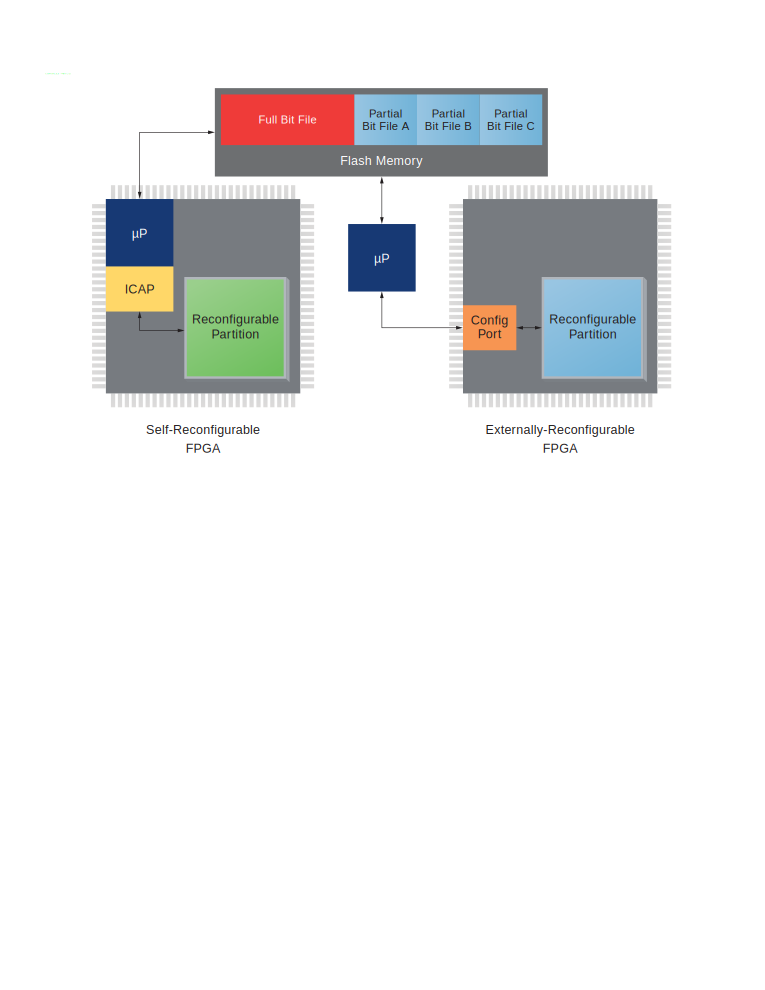
\includegraphics[width=0.8\textwidth]{fig/c1_introducao/reconf_externa.pdf}
\caption{Imagem ilustrativa para diferenciação entre autorreconfiguração e reconfiguração externa, extraido de \cite{wp374}.}
\label{fig:rexterna}
\end{figure}

É implicito o uso da reconfiguração parcial com a reconfiguração dinâmica, uma vez que faz pouco sentido reconfigurar todo o FPGA enquanto ela ainda está em execução.
Note que este tipo de reconfiguração em geral também necessita de uma parte permanentemente est\'atica, para interfacear com o circuito controlador.
Esta parti\c{c}\~ao est\'atica \'e respons\'avel pelo menos por controlar a comunica\c{c}\~ao com o circuito controlador.

Vale lembrar que a este tipo de reconfiguração, apesar de abrir muitas possibilidades, introduz uma necessidade de preocupação com \textit{overheads} de reconfiguração \cite{Hauck2007}.
Este \textit{overhead} é proporcional ao tamanho da partição que se deseja modificar e inversamente proporcional às velocidades das interfaces de reconfiguração.
Tal fator pode se tornar crucial na escolha entre o uso desta tecnologia ou alguma outra alternativa, possivelmente multiplexada.
Note que existem outros fatores que influenciam na opção por reconfiguração dinâmica, tais como preço, capacidade e potência, dentre outros, que não serão considerados aqui.

\subsection{Autorreconfigura\c{c}\~ao}
Modalidade de reconfigura\c{c}\~ao din\^amica parcial onde a reconfigura\c{c}\~ao do dispositivo \'e decidida por uma l\'ogica pertencente a ele mesmo.
Normalmente usa-se um microcontrolador ou uma m\'aquina de estados finitos para controlar a mudan\c{c}a de configura\c{c}\~oes.
Este tecnologia \'e nova e ainda representa uma forte \'area de pesquisa.
Por isso n\~ao s\~ao todos os FPGAs que d\~ao suporte a este tipo de reconfigura\c{c}\~ao.

Para que a autorreconfigura\c{c}\~ao aconte\c{c}a, os \textit{bitstreams}, resultado da sintetiza\c{c}\~ao, devem ser passados para uma mem\'oria acess\'i­vel ao FPGA durante a execu\c{c}\~ao do mesmo.
O circuito controlador identifica ent\~ao um padr\~ao que defina a necessidade de reconfigura\c{c}\~ao e transfere o \textit{bitstream} correspondente a esta nova necessidade para a parti\c{c}\~ao destino, que assim muda seu comportamento.
Note que para tal, as entradas e sa\'i­das das parti\c{c}\~oes tem que ser fixas, para que a mudan\c{c}a nas configura\c{c}\~oes das parti\c{c}\~oes n\~ao danifique o FPGA em si.

\section{Ferramentas}
Diversas ferramentas foram utilizadas para a realização deste trabalho.
Dentre eles pode-se citar os programas da Xilinx, interpretadores da linguagem Python, Perl e Tcl, compiladores de \LaTeX~e a ferramenta de controle de versão Git.
Abaixo segue uma pequena descrição sobre as ferramentas mais críticas destas.

\subsection{Xilinx ISE Design Suite}
O \textit{ISE Design Suite} é um conjunto de ferramentas da Xilinx para o desenvolvimento de projetos de \textit{hardware}.
Estes programas estão apresentados a seguir.

\subsubsection{Xilinx ISE Design Tools}
O \textit{ISE Design Tools}, disponível para os sistemas Windows XP (32 e 64 bits), Windows 7 (32 e 64 bits), Windows Server 2008 (64 bits), Red Hat Enterprise 5 e 6 (32 e 64 bits) e SUSE Linux Enterprise 11 (32 e 64 bits) \cite{ug631}, controla todos os aspectos do fluxo de projeto \cite{ug695}.
Através do \textit{Project Navigator}, sua principal ferramenta, é possivel acessar todas as configurações e ferramentas de implementação de configurações.

\paragraph{\textit{Project Navigator}} O \textit{Project Navigator} é a principal ferramenta do \textit{ISE Design Tools}.
Através dela é possível criar projetos, incluir arquivos de descrição de \textit{hardware}, seja em VHDL, Verilog ou esquemáticos, construir componentes de propriedade intelectual, impor restrições e compilá-los, dentre outras coisas.
Em geral, todo o desenvolvimento começa através desta ferramenta para fins de verificação de lógica.

\paragraph{iMPACT}
O iMPACT é utilizado para se construir arquivos para a inicialização de memórias Flash e para a programação de FPGAs e suas memórias.
Ele pode ser acessado por linha de comando, permitindo que outras ferramentas incorporem suas funções.

\paragraph{\textit{CORE Generator}}
O \textit{CORE Generator} é uma ferramenta muito útil, utilizada para a construção de blocos lógicos prontos de funções variadas.
Em geral, seus blocos instanciam algum componente de propriedade intelectual da Xilinx.

\subsubsection{\textit{Embedded Development Kit}}
O \textit{Embedded Development Kit} é um conjunto de ferramentas voltados para o desenvolvimento de sistemas microprocessados embarcados em FPGA.

\paragraph{\textit{Xilinx Platform Studio}}
A \textit{Xilinx Platform Studio} permite a construção de sistemas microprocessados.
Ela possui uma gama muito grande de componentes periféricos que podem acrescentados a este sistema e integrados de forma automática ou manual.

\paragraph{\textit{Xilinx Software Development Kit}}
Com as informações do sistema microprocessado, é possível utilizar \textit{Xilinx Software Development Kit} para a criação do programa que será embarcado.
Esta ferramenta permite a programação do dispositivo, bem como da memória Flash, com ou sem o programa já adicionado, tornando-se uma ferramenta muito simples e útil.

\subsubsection{PlanAhead}
O PlanAhead é uma das ferramentas mais poderosas de toda a \textit{suite}.
Ele permite que projetos sejam integrados e pré-alocados em FPGAs, bem como gerenciar, modificar e verificar restrições de tempo, alocação e mapeamento, dentre outros.
Ele permite ainda que módulos reconfiguráveis sejam acrescentados ao projeto, tornando a reconfiguração dinâmica um problema bem mais acessível.

\subsubsection{Ferramentas de Linha de Comando}
Além de todas as ferramentas já apresentadas, a plataforma da Xilinx ainda oferece ferramentas de linha de comando, acessadas pelo \textit{prompt} to Windows.
Através destas ferramentas é possível realizar qualquer tarefa realizavel pela ferramentas com interface gráfica e mais algumas outras.
Abaixo menciona-se a ferramenta mais importante e mais utilizada deste conjunto.

\paragraph{Xilinx Sinthesis Tool (XST)}
A XST é o equivalente ao compilador para a programação convencional.
Ele realiza verificações léxicas e sintáticas dos arquivos para gerar na saída algum arquivo compilado, tipicamente NGC ou BIT.

\ifx\compilewholereport\undefined
	\bibliographystyle{authordate1} 
	\newsavebox\mytempbib\savebox\mytempbib{\parbox{\textwidth}{\bibliography{bibliografia}}}
	%\listoftodos
	\end{document}
\fi